\chapter{Implementacja systemu}
\thispagestyle{chapterBeginStyle}

W tym rozdziale opisane są szczegóły implementacyjne projektu. Więcej uwagi poświęcono urządzeniom wchodzącym w skład systemu oraz opisano użyte technologie, wraz z uargumentowaniem, dlaczego to właśnie one zostały wybrane. Kolejnym elementem jest omówienie struktury projektu oraz wypunktowania, co znajduje się w poszczególnych plikach z kodem źródłowym. Zaprezentowano na przykładzie wynik działania systemu, opisano problemy napotkane w trakcie pracy oraz przedstawiono sposób prowadzenia projektu.

\section{Opis urządzeń}

\subsection{Raspberry Pi}
Programy wykonywane są na urządzeniach z rodziny Raspberry Pi \cite{RPi}. Są to jednopłytkowe minikomputery, tzw. SoC (ang. \textit{System-on-a-chip}). Ich jednostką obliczeniową jest procesor firmy Broadcom, wykonany w architekturze ARM. Pozwalają na obsługę i komunikację z innymi urządzeniami za pomocą wielu portów i interfejsów: m.in. USB, HDMI, GPIO (40 pinów wejścia/wyjścia ogólnego przeznaczenia), CSI (interfejs kamery), RJ-45, Wi-Fi czy Bluetooth. Nie posiadają one wbudowanej pamięci, wszystkie dane są zapisywane na karcie SD, na której znajduje się również system operacyjny, najczęściej Linux. Organizacja produkująca minikomputery wydaje swoją dystrybucję nazwaną Raspberry Pi OS (wcześniej Raspbian), opartą na Debianie. Wydanych zostało kilka wersji Raspberry różniących się od siebie przeznaczeniem i specyfikacją. W systemie użyto \verb|Pi 4| i \verb|Pi Zero|. Pierwsza z nich to najnowsza wersja, z czterordzeniowym procesorem taktowanym zegarem 1,5 GHz oraz pamięcią RAM 2 GB. Druga zaś jest odpowiedzią na sytuacje, gdzie tak duże moce obliczeniowe nie są potrzebne -- Pi Zero ma mniejsze wymiary, słabszy procesor oraz mniej pamięci RAM, co skutkuje również mniejszą ceną.
\subsection{Kamery}
Kamery użyte w systemie to kamery dedykowane do Raspberry Pi: Camera Module v1 z matrycą OmniVision OV5647. Pozwalają na wykonywanie zdjęć w rozdzielczości 2592 $\times$ 1944 pikseli, ich poziome pole widzenia to $53,5 \degree \pm 0,13 \degree$, a ogniskowa wynosi 3,60 mm. Pełna specyfikacja jest dostępna na stronie producenta \cite{RPi}.

Początkowo planowano użycie jedynie jednego minikomputera, do którego podłączone byłyby dwie kamery USB lub jedna kamera Pi i jedna USB. Pierwszy wariant został odrzucony z powodu wysokiej ceny (lub gorszej jakości) kamer internetowych oraz możliwymi problemami z przepustowością USB. Drugi za to wprowadzałby niepotrzebny brak spójności oraz niemożność reużywania kodu źródłowego, obsługującego kamerę dedykowaną. Dodatkowo, tego typu kamera posiada sprzętowe i programowe wsparcie i oferuje pełną kompatybilność z urządzeniem, co wpływa na szybkość i niezawodność działania. Niemożliwe jest jednak bezpośrednie podłączenie dwóch takich kamer, gdyż \verb|Pi 4| posiada jedynie jeden port CSI. Dlatego zdecydowano się na użycie drugiego, tańszego urządzenia z serii Raspberry, do którego można podłączyć drugą kamerę. 
\clearpage
\section{Technologie}
Użyte technologie:
\begin{itemize}
  \item Python 3.7
  \item OpenCV 4.1.0
  \item picamera 1.13
  \item WebSocket
  \item JavaScript ES6
  \item React Native 0.63
  \item Expo 39
\end{itemize}

Kod źródłowy uruchamiany na obu urządzeniach Raspberry został napisany w języku Python 3.7. Został on wybrany z powodu jego prostoty oraz istnienia wielu bibliotek specyficznych dla minikomputera, które napisane są właśnie w tym języku. Wspiera on wiele paradygmatów programowania, dzięki czemu programista ma swobodę w wyborze sposobu implementacji rozwiązań. Automatyczne zarządzanie pamięcią zmniejsza ryzyko błędów, a sprawdzone biblioteki do operacji macierzowych zapewniają szybkość działania.

Do przetwarzania obrazu użyto biblioteki OpenCV, która dostarcza wiele gotowych modułów do rozwiązywania najczęstszych problemów związanych z widzeniem komputerowym, zapewniając jednocześnie duże możliwości konfiguracji, poprzez dobieranie parametrów. Biblioteka napisana jest w języku C++, ale posiada nakładki pozwalające na wywoływanie funkcji z poziomu innych języków, m.in. Pythona.

Wykonywanie zdjęć za pomocą kamery dedykowanej do Raspberry Pi byłoby trudne bez interfejsu, który dostarcza metody umożliwiające kontrolę pracy kamery na wysokim poziomie abstrakcji, bez wnikania w szczegóły jej budowy. Rolę tego interfejsu pełni picamera \cite{picamera}, moduł napisany w Pythonie specjalnie do tego celu. Pomimo prostoty użytkowania, daje możliwość zmiany wielu parametrów wpływających na zdjęcie, takich jak: czas naświetlania, liczba klatek na sekundę, rozdzielczość czy balans bieli. Dokumentacja opisuje sposób na przekształcenie zdjęć do formatu zgodnego z wymaganiami OpenCV.

Komunikacja pomiędzy serwerem a aplikacją mobilną odbywa się z użyciem protokołu WebSocket. Po stronie aplikacji wsparcie dla tego sposobu komunikacji jest wbudowane, lecz w języku Python należy wybrać jedną z szeregu zewnętrznych bibliotek, w których można stworzyć serwer. Implementacja została oparta o niewielką i mało popularną bibliotekę SimpleWebSocketServer \cite{SimpleWebSocket}, która jest jednak wystarczająca do obecnych potrzeb. 

Do wykonania aplikacji klienckiej użyto platformy programistycznej React Native \cite{ReactNative}, dzięki której za pomocą jednej wersji kodu źródłowego tworzy się aplikację kompatybilną zarówno z systemem Android, jak i iOS. Z powodu bardzo dużych podobieństw do biblioteki React.js i używania języka JavaScript, tworzenie oprogramowania jest bardzo podobne do tworzenia aplikacji webowej. Środowisko Expo \cite{expo} zapewnia za to narzędzia pomocne w rozwijaniu, budowaniu i uruchamianiu aplikacji. Dzięki niemu możliwe jest używanie aplikacji mobilnej również przez przeglądarkę internetową. Wieloplatormowość to zdecydowany atut aplikacji.

\section{Struktura projektu}
\label{structure}
\begin{forest}
for tree={font=\sffamily, grow'=0,
folder indent=.9em, folder icons,
edge=densely dotted}
[pi-darts
  [app
      [src
          [assets
              [dartboard.svg, is file]]
          [components
              [Dartboard.js, is file]]
          [helpers
              [WebSocketClient.js, is file]]
          [App.js, is file]]
      [app.json, is file]
      [package.json, is file]]
  [rpi
      [src
          [main$\_$pi4.py, is file]
          [main$\_$pi0.py, is file]
          [app$\_$connector.py, is file]
          [pi$\_$connector.py, is file]
          [camera.py, is file]
          [throw$\_$detector.py, is file]
          [triangulation.py, is file]
          [board$\_$mapping.py, is file]]
      [sync.sh, is file]
      [requirements.txt, is file]]
]
\end{forest}

Folder z projektem o nazwie \verb|pi-darts| zawiera dwie aplikacje: \verb|app| i \verb|rpi|. Pierwsza z nich jest jest uruchamiana na smartfonie, druga na \verb|Pi 4| i \verb|Pi 0|.

\subsubsection{Opis plików źródłowych}
\begin{itemize}
  \item \verb|main_pi4.py| -- główny skrypt uruchamiany na \verb|Pi 4|, konfiguruje pozostałe moduły i zawiera główną pętlę programu.
  \item \verb|main_pi0.py| -- główny skrypt uruchamiany na \verb|Pi Zero|, bardzo podobny do \verb|main_pi4.py|. Również zawiera pętlę, w której wykonywane są nieustannie zdjęcia, lecz nie zajmuje się komunikacją z aplikacją.
  \item \verb|app_connector.py| -- zawiera klasę serwera aplikacji, dostarcza interfejs do wystartowania serwera w osobnym wątku oraz wysyłania komunikatów do klientów.
  \item \verb|pi_connector.py| -- używany przez oba urządzenia w celu ustanowienia połączenia. Składa się z dwóch klas: jednej dla serwera (\verb|Pi 4|), z metodami do uruchomienia gniazda TCP i przyjęcia wiadomości, a drugiej dla klienta (\verb|Pi Zero|), z funkcjami do podłączenia się do serwera oraz wysłania komunikatu.
  \item \verb|camera.py| -- dodatkowy interfejs opakowujący metody biblioteki \verb|picamera|. Daje możliwość wstępnego ustawienia kamery oraz wykonania zdjęcia reprezentowanego w formacie zgodnym z OpenCV.
  \item \verb|throw_detector.py| -- moduł, w którym zaimplementowana jest logika wykrywania rzutu. W tym miejscu wykonywane są wszystkie operacje na obrazach.
  \item \verb|triangulation.py| -- plik, w którym zapisane są funkcje przeprowadzające triangulację
  \item \verb|board_mapping.py| -- komponent przyporządkowujący pozycję rzutki we współrzędnych kartezjańskich do konkretnego pola na rzutce
  \item \verb|App.js| -- główny komponent aplikacji mobilnej. Zarządza jej stanem oraz przekazuje informacje do \verb|Dartboard.js|.
  \item \verb|Dartboard.js| -- komponent ze graficznym przedstawieniem tarczy, umożliwia zaznaczanie miejsca wbicia rzutki.
  \item \verb|WebSocketClient.js| -- pomocniczy plik ustanawiający połączenie oraz przyjmujący komunikaty z serwera za pomocą technologii WebSocket.
  
\end{itemize}

\section{Efekt końcowy}
Efekty działania aplikacji zostaną pokazane na przykładzie. Na rysunku \ref{rzutka_gora} widoczny jest rzut z góry na tarczę z wbitą rzutką w pole standardowe 10. Następnie, na rysunku \ref{rzutka_kontury} zielonym kolorem zaznaczone zostały kontury wokół rzutki, osobno dla każdej z kamer. Pojedynczy, czerwony punkt jest uznawany za miejsce wbicia lotki. Ostateczny rezultat działania systemu widoczny jest na zrzucie ekranu z aplikacji mobilnej, gdzie prezentowane dane dobrze odzwierciedlają wykonany rzut.
\begin{figure}[h!]
\begin{center}
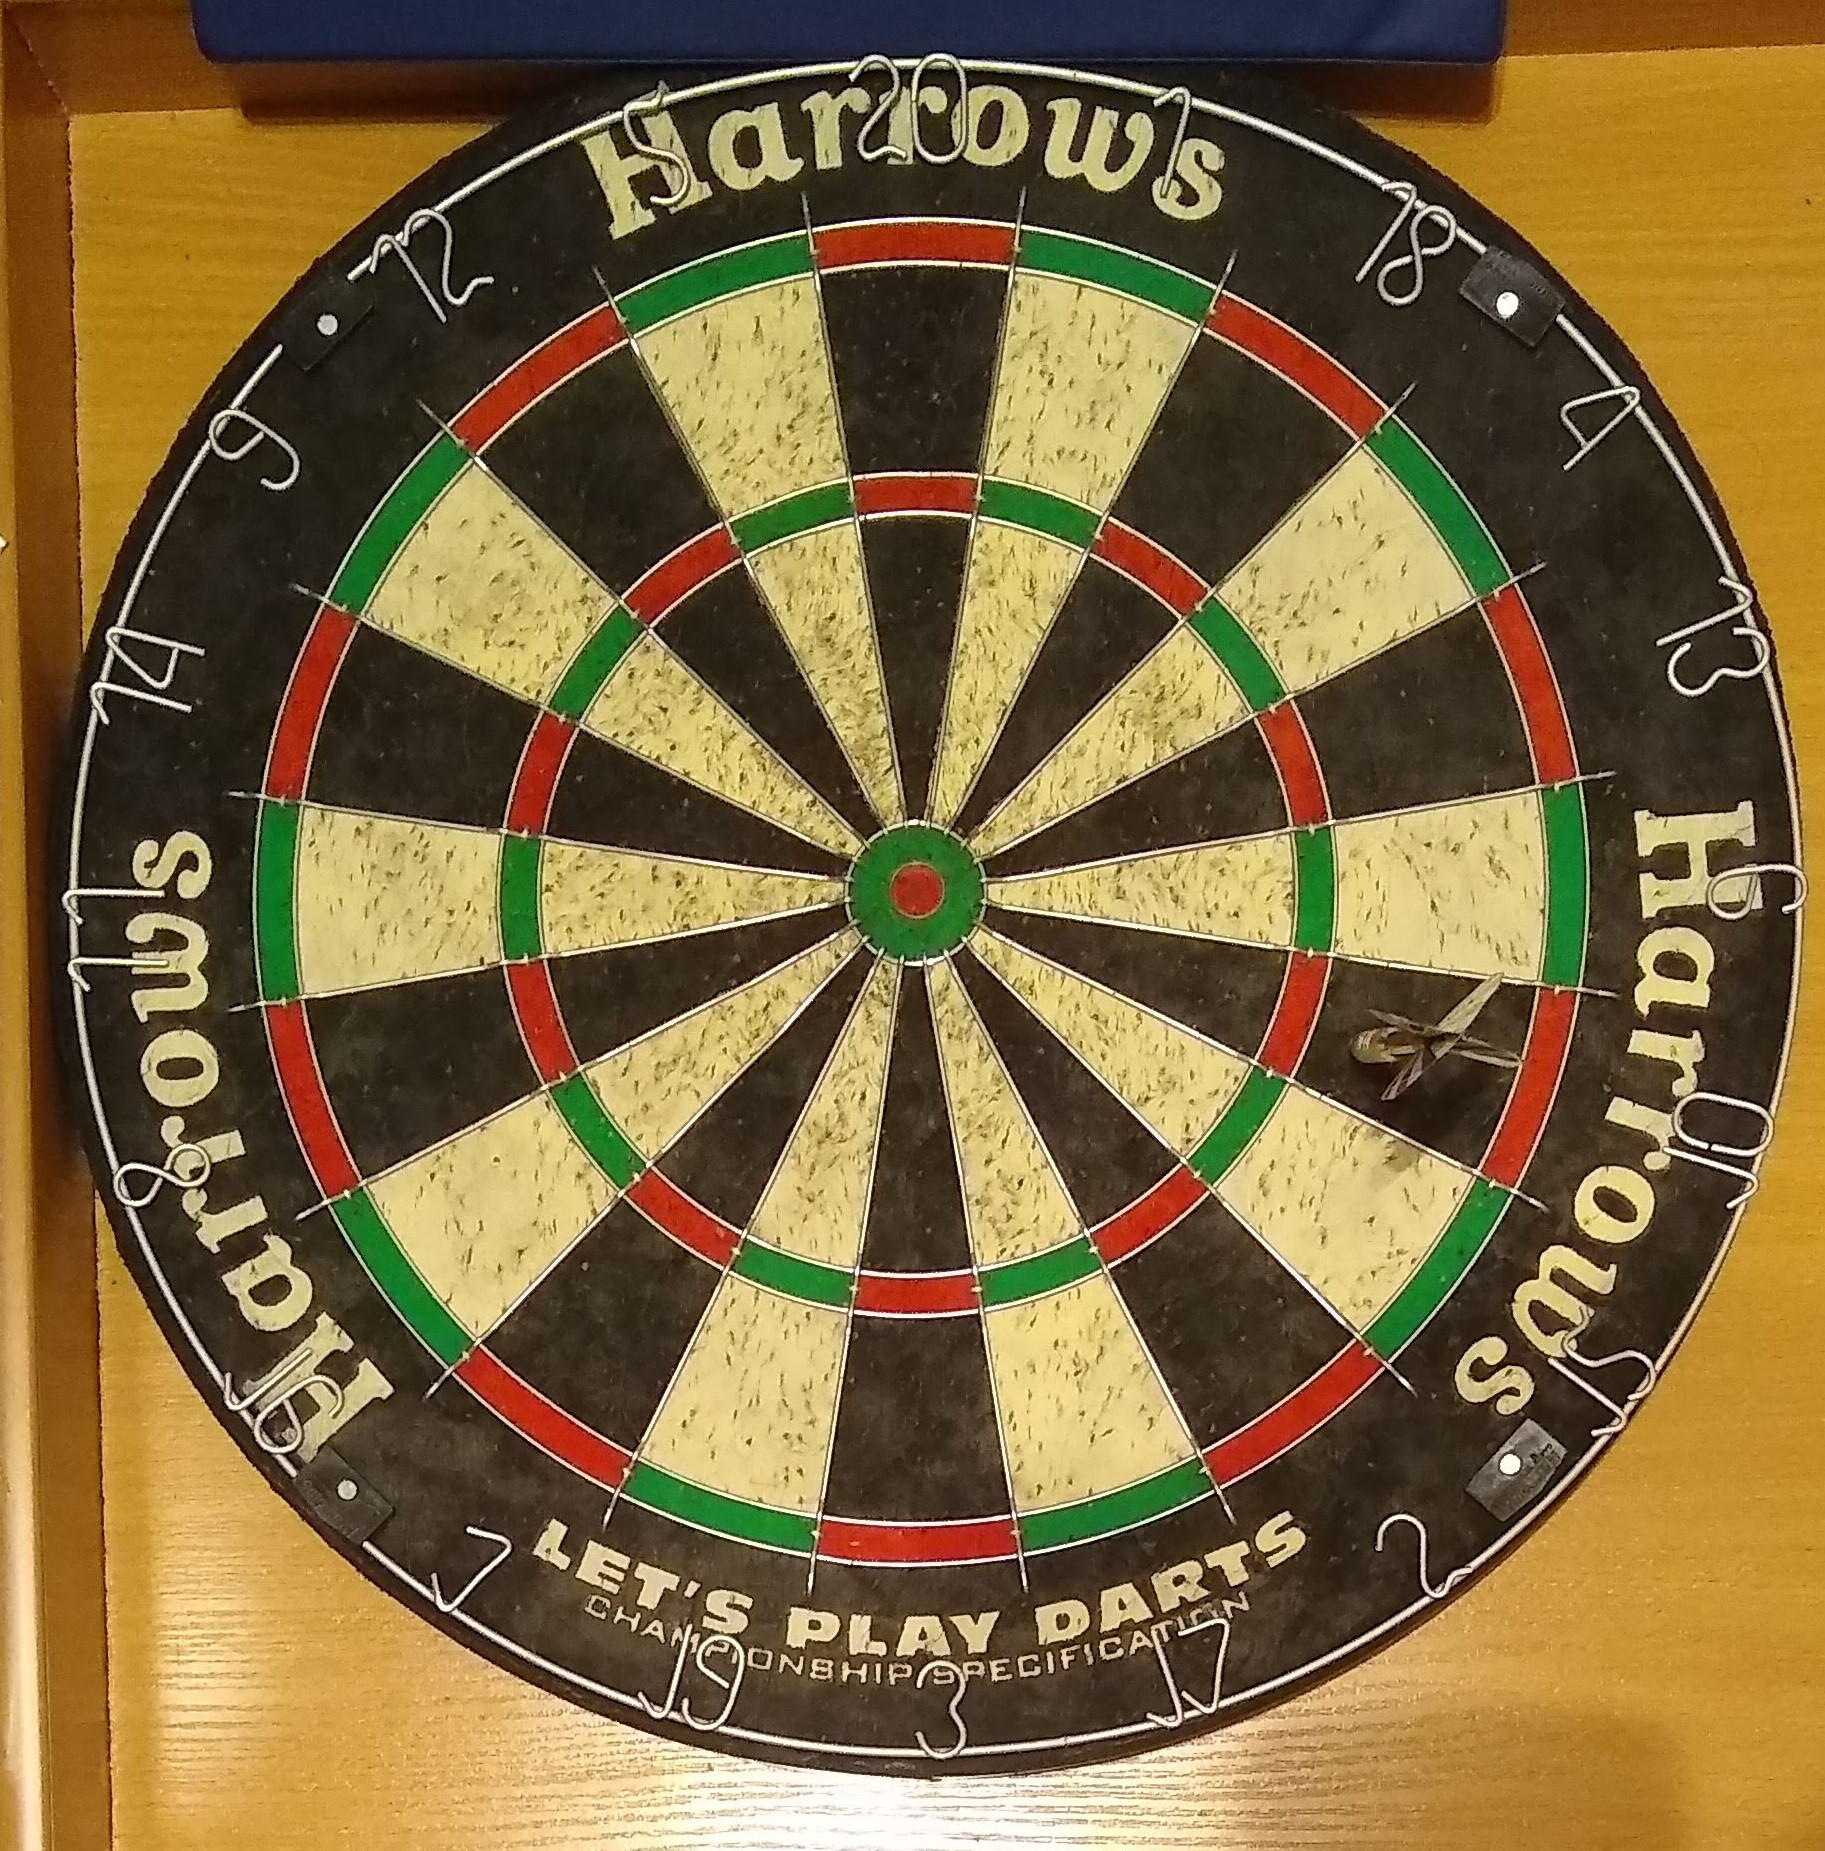
\includegraphics[width=0.5\textwidth]{obrazki/rzutka_gora.jpg}
\end{center}
\captionsource{{\color{dgray}Rzutka wbita w tarczę (rzut z góry)}}{Opracowanie własne}
\label{rzutka_gora}
\end{figure} 

\begin{figure}[h!]
\centering
\begin{subfigure}{\textwidth}
  \centering
  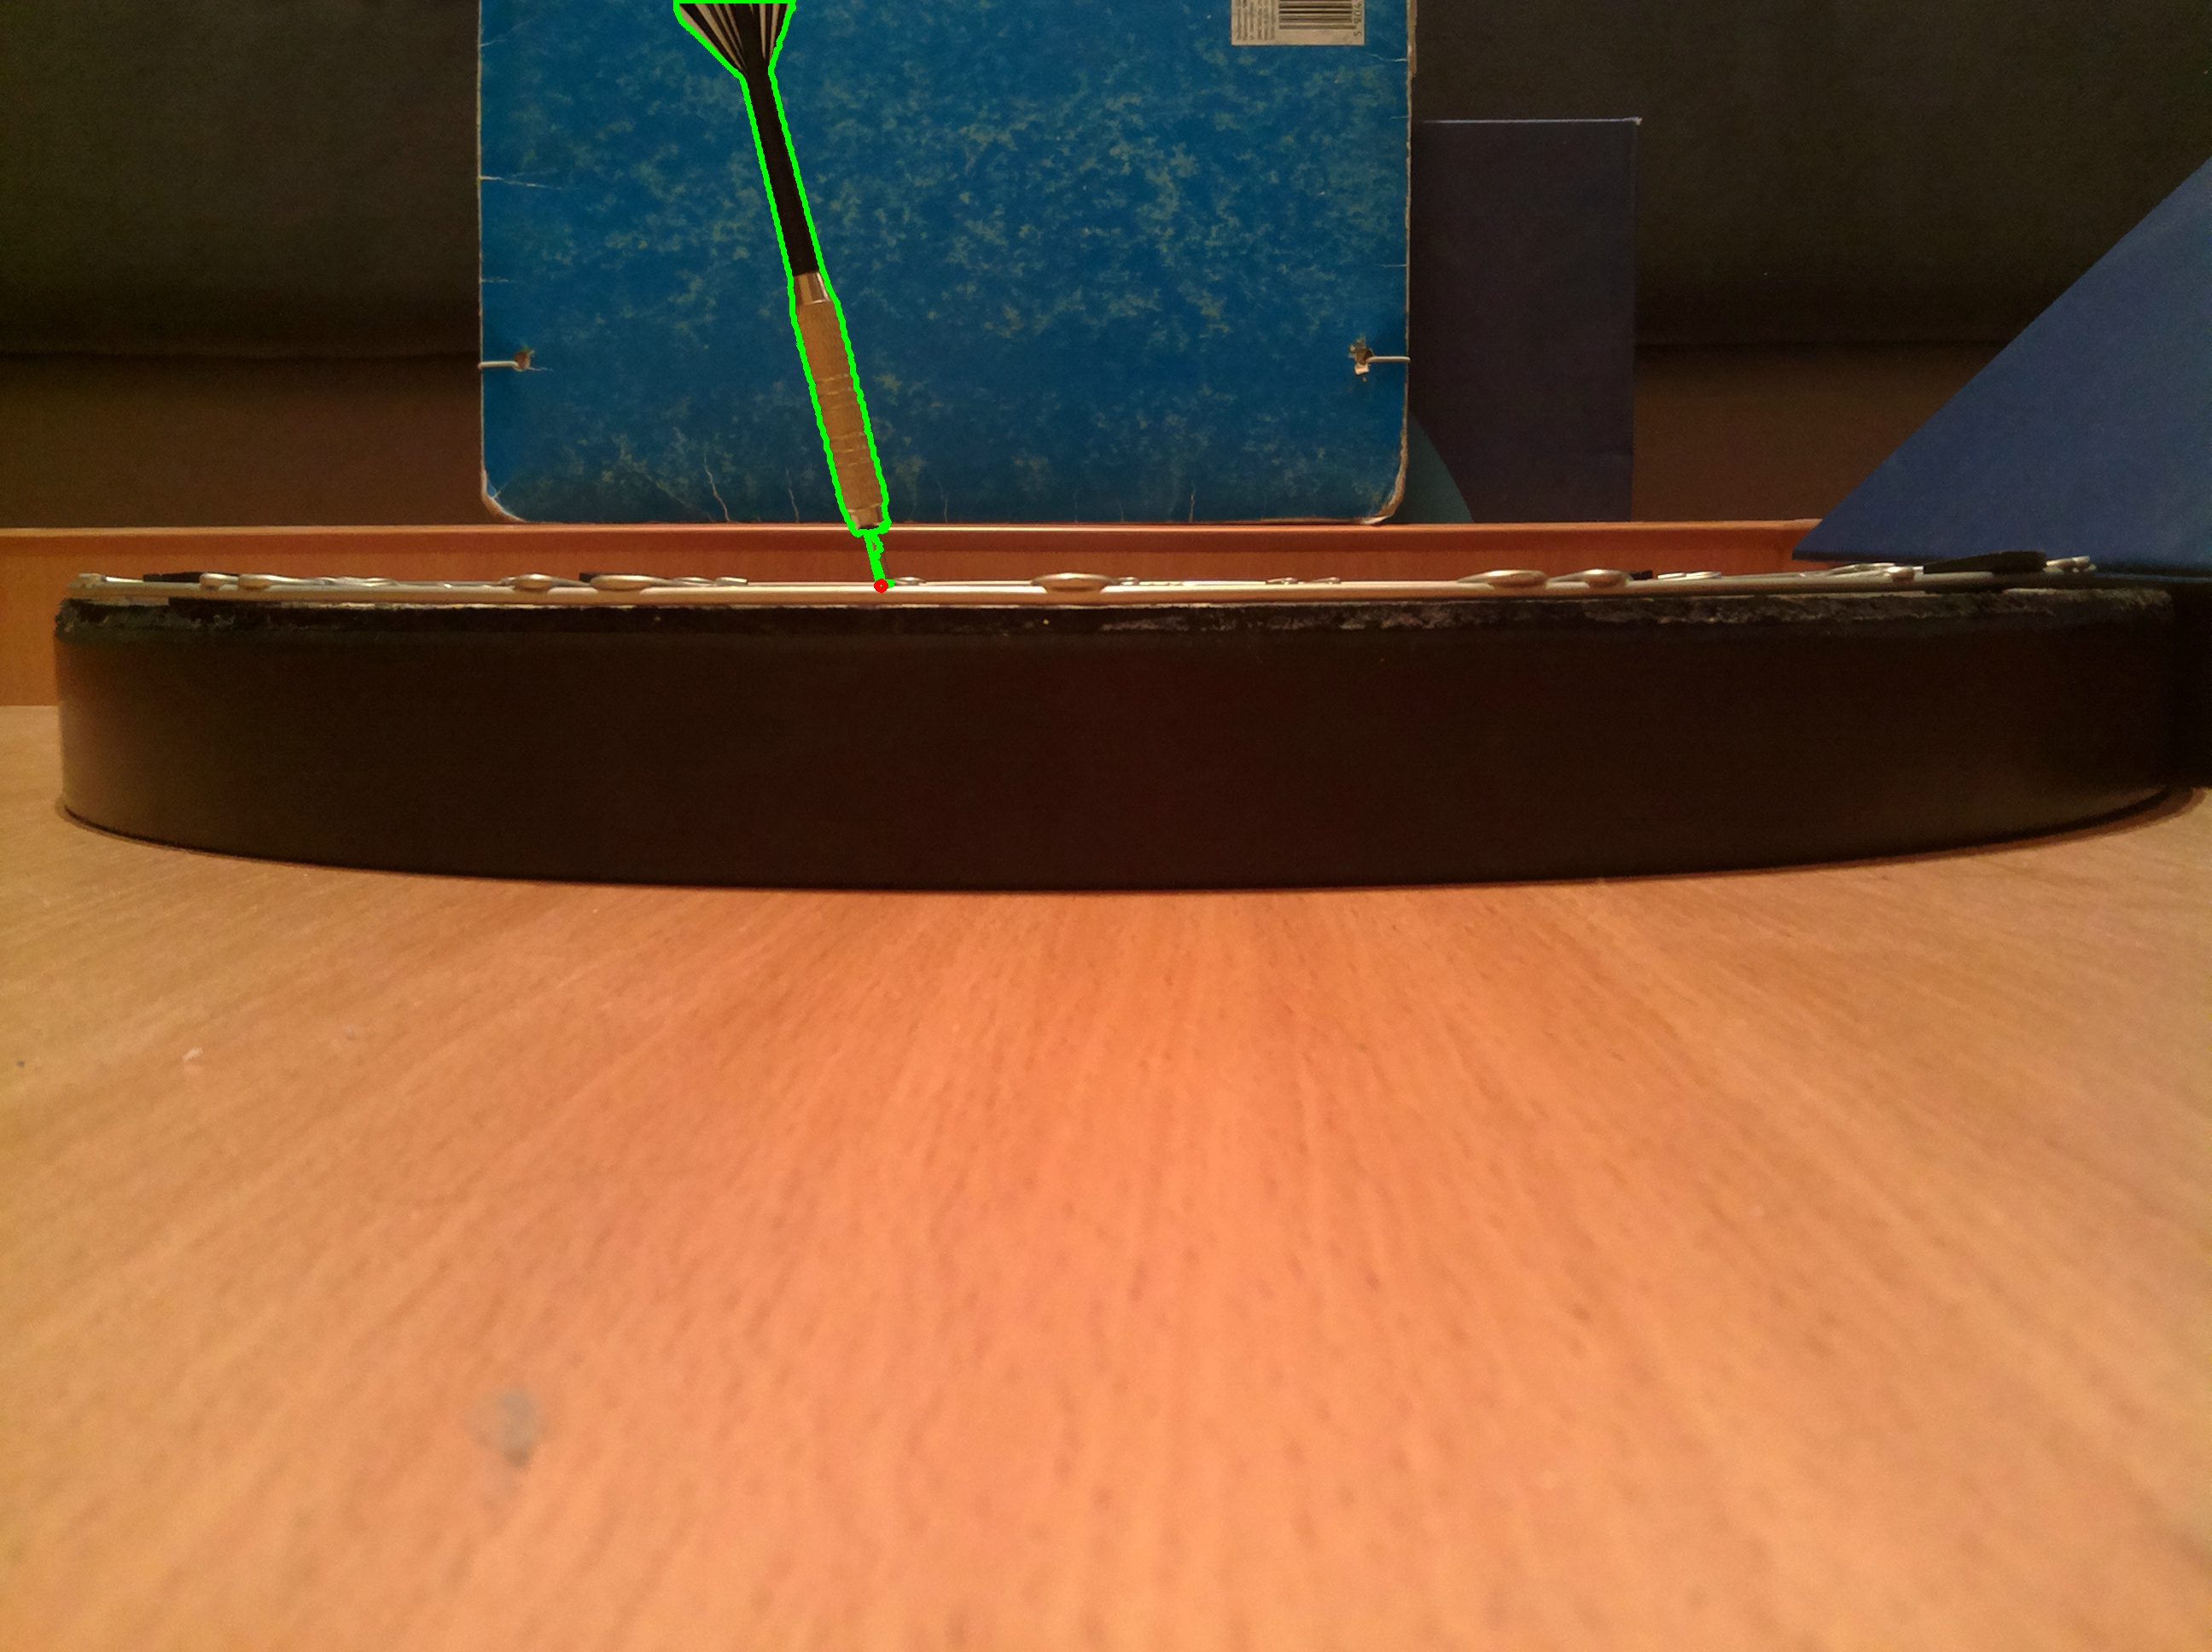
\includegraphics[width=0.75\textwidth]{obrazki/rzutka_pi0.jpg}
  \captionsource{{\color{dgray}Widok z prawej kamery}}{Opracowanie własne}
  \label{rzutka_pi0}
\end{subfigure}
\begin{subfigure}{\textwidth}
  \vspace{0.5cm}
  \centering
  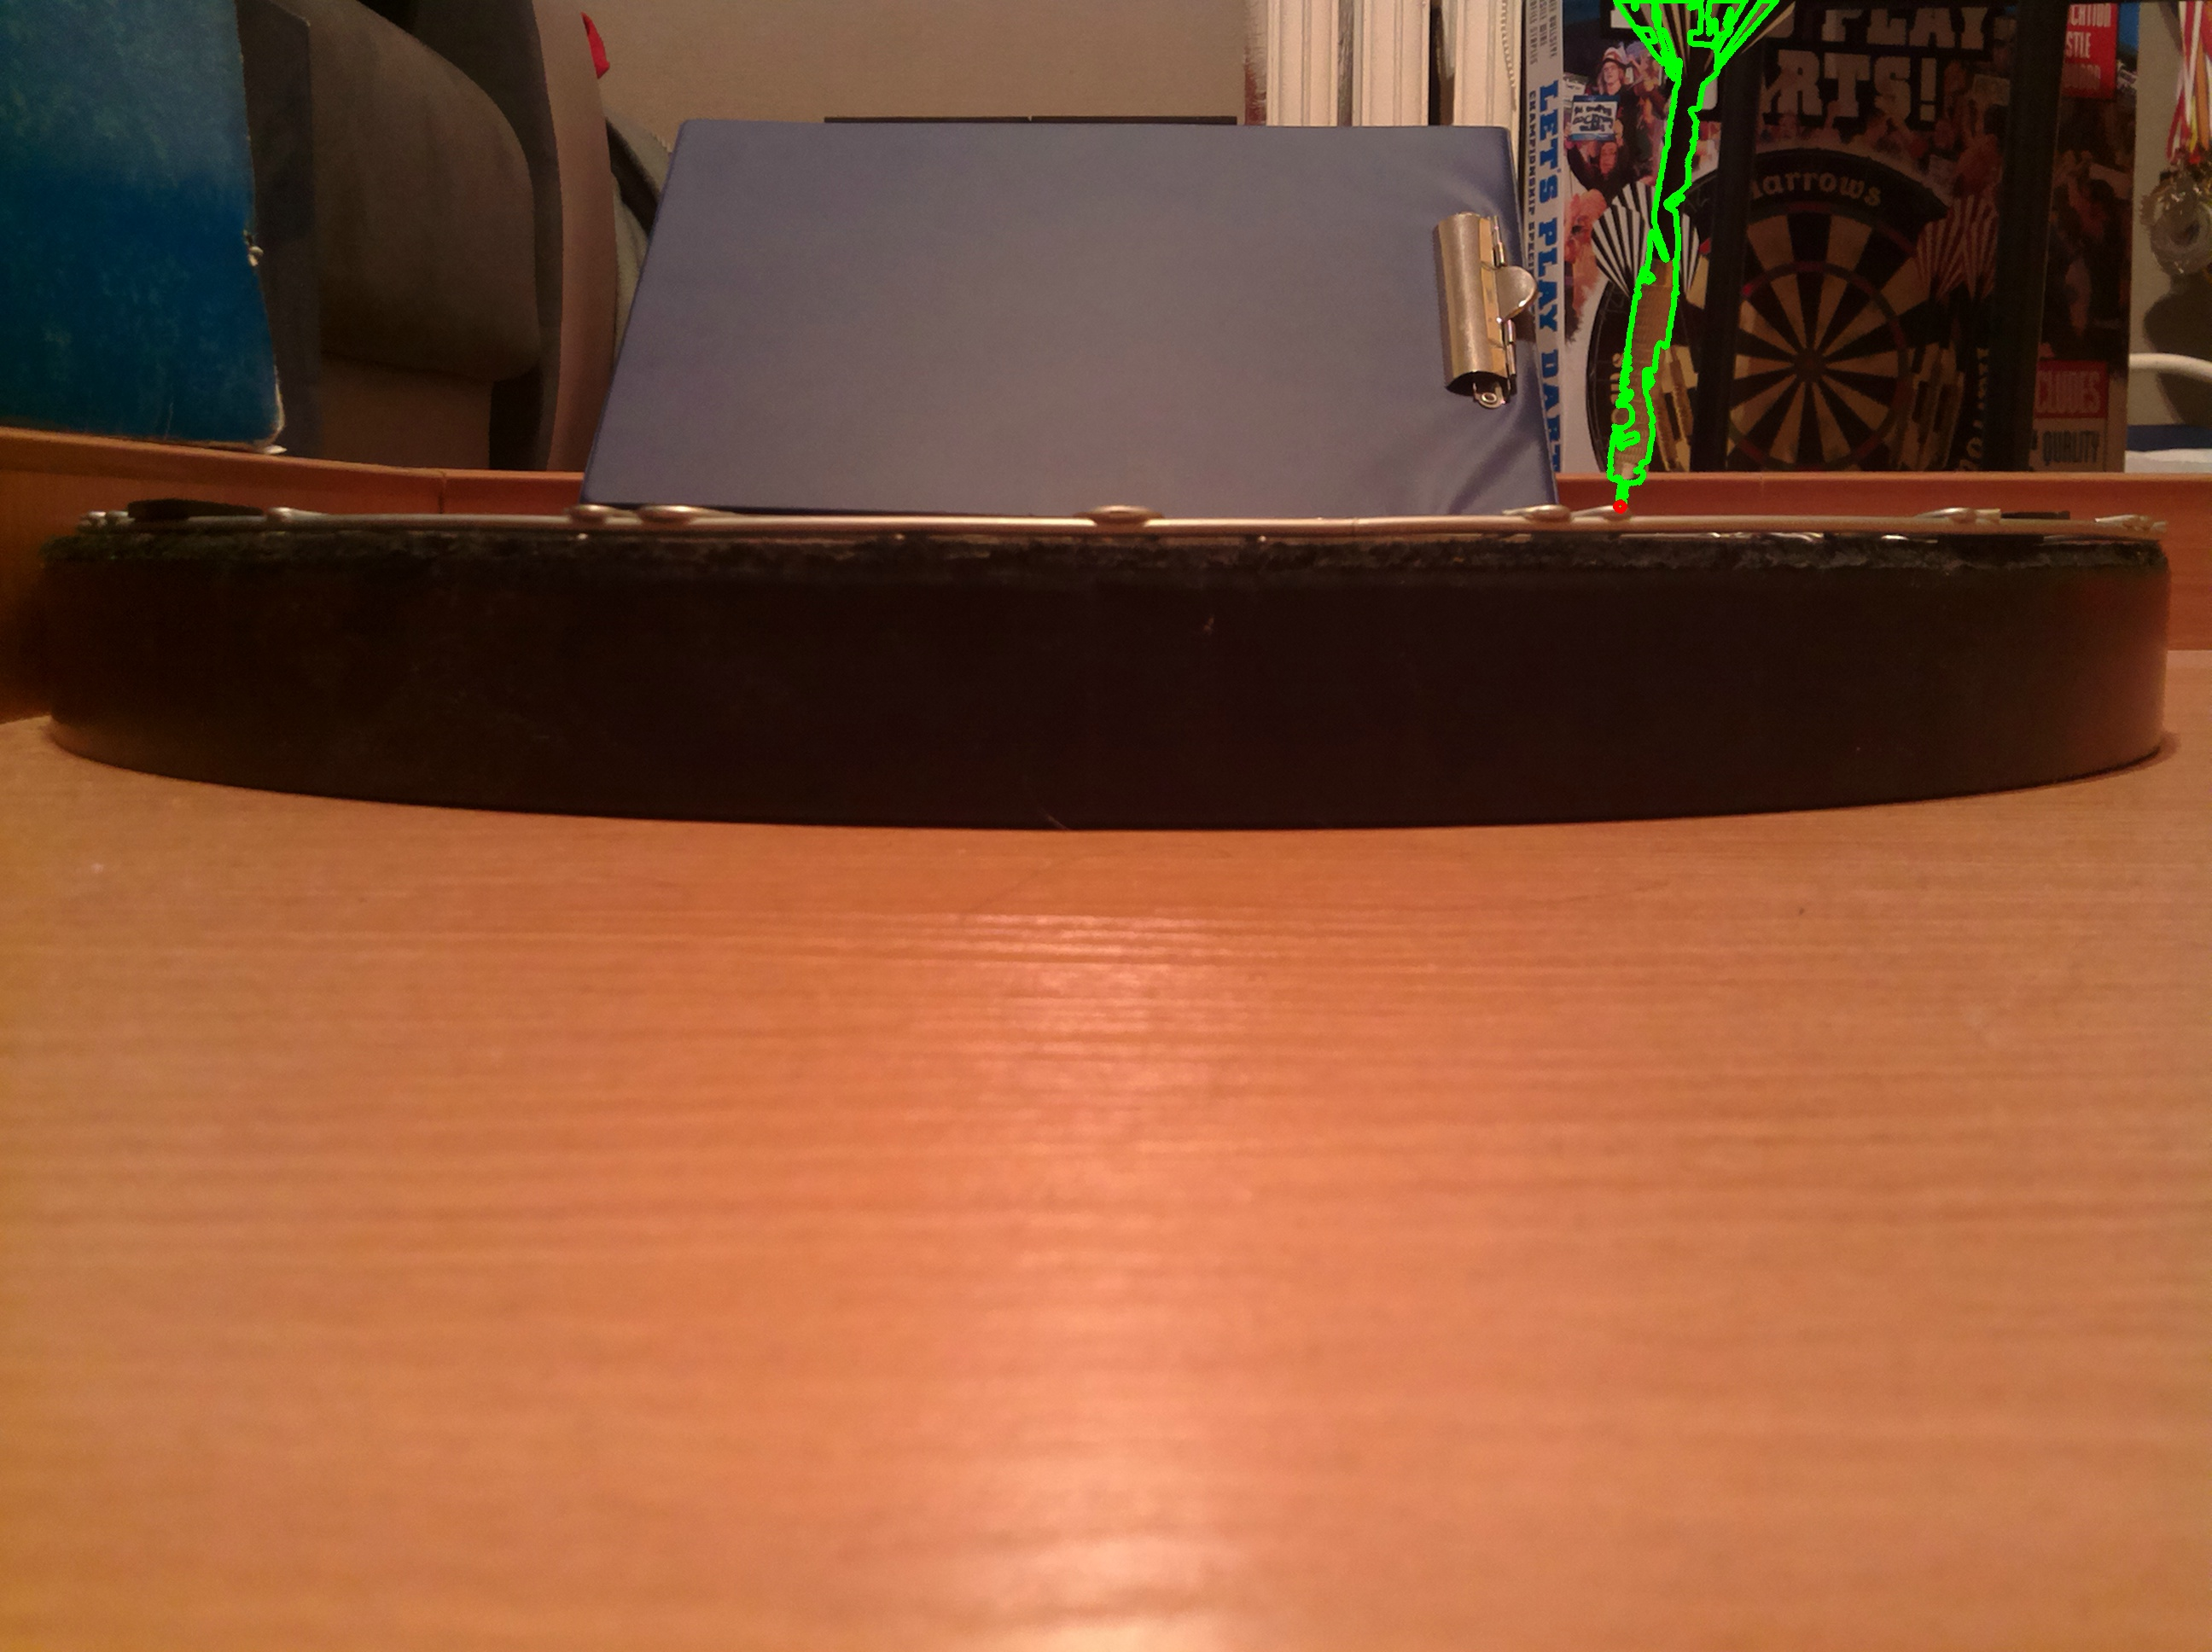
\includegraphics[width=0.75\textwidth]{obrazki/rzutka_pi4.jpg}
  \captionsource{{\color{dgray}Widok z dolnej kamery}}{Opracowanie własne}
  \label{rzutka_pi4}
\end{subfigure}
\caption{Wykrycie konturu rzutki}
\label{rzutka_kontury}
\end{figure}

\begin{figure}[h!]
\begin{center}
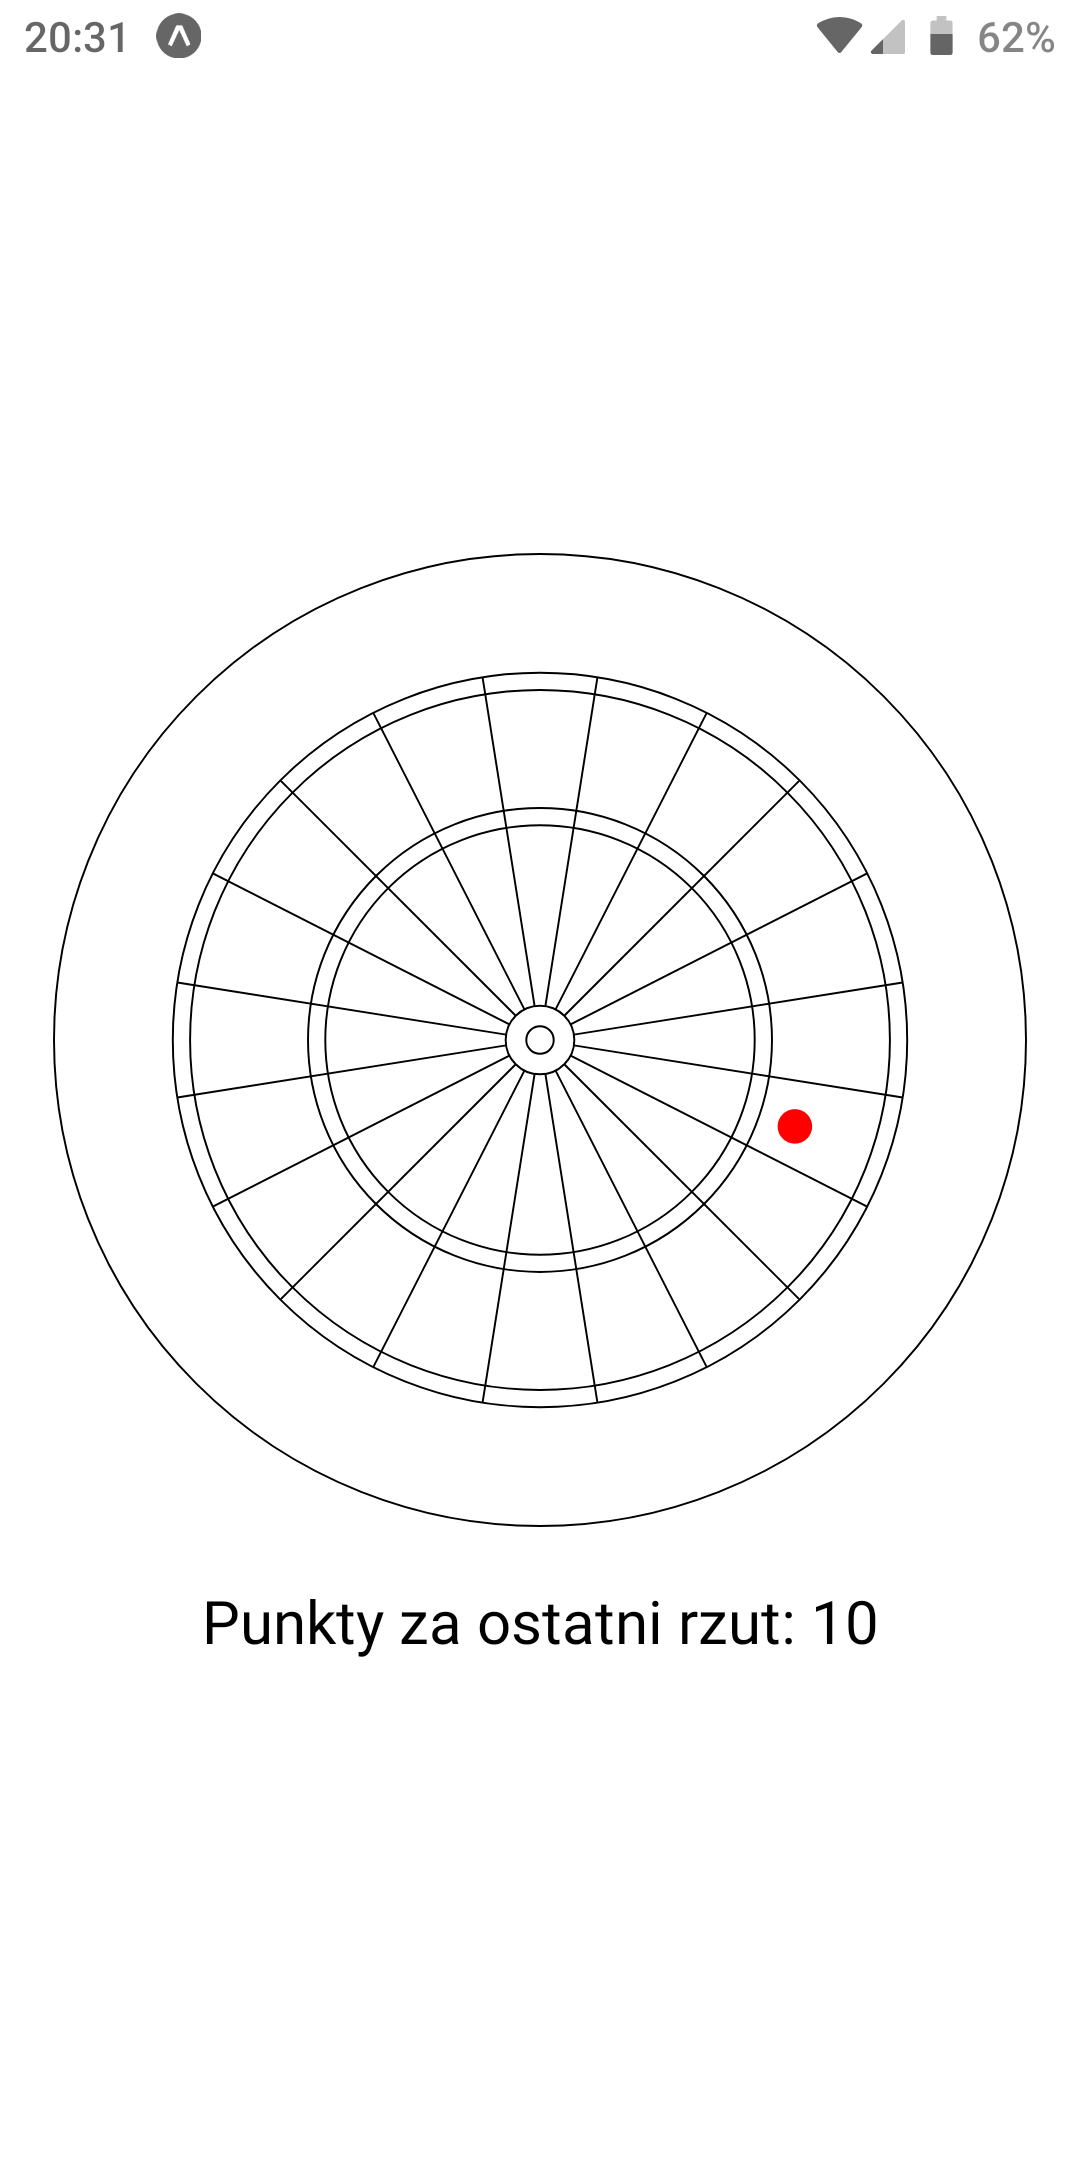
\includegraphics[width=0.3\textwidth]{obrazki/screenshot.png}
\end{center}
\captionsource{{\color{dgray}Zrzut ekranu z aplikacji mobilnej}}{Opracowanie własne}
\label{screenshot}
\end{figure} 

\section{Testy}
Po skończeniu implementacji, wykonano testy dokładności wykrywania pozycji rzutki. Przeprowadzono 20 tur rzutów po 3 rzuty oraz sprawdzono, jaki procent z nich został poprawnie rozpoznany. Wyniki przestawia tabela \ref{table:testy}. Łatwo zauważyć, że przy pierwszym rzucie w turze wyniki są zadowalające, lecz z każdym kolejnym rzutem są coraz niższe. Wynika to m.in. z sytuacji, gdy jedna lotka przesłania drugą, utrudniając analizę. Rozwiązaniem tego problemu jest np. dodanie kolejnej kamery.
\begin{table}[h!]
\begin{tabular}{|l|l|l|l|}
\hline
Rzut 1 & Rzut 2 & Rzut 3 & Łącznie \\ \hline
90\%   & 75\%   & 55\%   & 73,34\% \\ \hline
\end{tabular}
\captionsource{{\color{dgray}Wyniki testów }}{Opracowanie własne}
\label{table:testy}
\end{table}
\section{Problemy}
Podczas tworzenia systemu natrafiono na szereg problemów, m.in:
\begin{itemize}
  \item ograniczone zasoby \verb|Raspberry Pi Zero|, powodujące przerywanie programu przy dużym obciążeniu.
  \item mało skuteczne wykrywanie rzutki, gdy tło miało podobny kolor do koloru lotki. Z tego powodu za stelażem ustawiono prowizoryczne zasłony o odmiennych kolorach. Przez długi czas skuteczność obniżała również zbyt wczesna (tj. wykonana przed odjęciem tła) konwersja obrazu do skali szarości, powodująca stratę informacji.
  \item instalacja biblioteki OpenCV, która (w przypadku kompilacji bezpośrednio ze źródeł), trwała na \verb|Pi Zero| ok. 20 godzin.
  \item ustawienie rozdzielczości zdjęcia -- okazało się, że szerokość i wysokość muszą być wielokrotnościami 16.
  \item słaba jakość zdjęć -- przed użyciem i poprawną konfiguracją picamera, zdjęcia wykonywane w trakcie działania systemu były wyraźnie gorszej jakości niż te, wykonane statycznie, np. programem \verb|raspistill|.
\end{itemize}
\section{Prowadzenie projektu}
Projekt był tworzony z użyciem systemu kontroli wersji Git, a zdalne repozytorium znajduje się na portalu GitHub \footnote{Adres: \url{www.github.com}}. Umożliwiło to wygodną, jednoczesną pracę nad różnymi elementami programu, a także zapewniało bezpieczeństwo w przypadku ewentualnych pomyłek.

W celu udokumentowania procesu analizy i tworzenia systemu, a także wykonania implementacji na czas, wykorzystano funkcjonalności portalu GitHub do tworzenia tablic projektowych (ang. \textit{Kanban board}), do których systematycznie były dołączane nowe zadania. Wyznaczano również kamienie milowe, które wskazywały, w jakim miejscu znajduje się projekt. 